\section{Representação de não-linearidades}

Serão analisado o comportamento da rede frente a elementos resistivos não lineares. Essa análise é interessante para estuda de pára-raios, que controla, as sobretensões em sistemas de potência.

O modelo de linha segue a imagem abaixo:

\begin{figure}[H]
\begin{center}
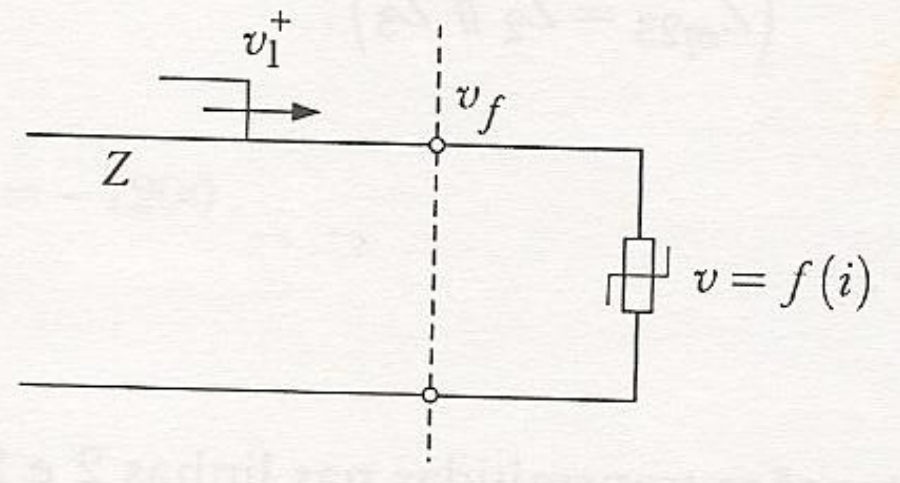
\includegraphics[width=8cm]{images/nlin.png}
\caption{Linha terminada com pára-raios.}
\label{slide7:nlin} 
\end{center}
\end{figure}

Pára-raios convencionais possuem centelhador em série com o resistor para saturar a tensão em um valor de sobretensão específico, com a finalidade de proteger o circuito. O exemplo tratado aqui não irá considerar tal centelhador.

A tensão incidente e a impedância características da linha podem ser representados por seu equivalente de Thèvenin, resultando em uma fonte de tensão de valor $2v_1^{+}$ seguida de uma impedância série $Z_1$ e que por fim se conecta ao pára-raios.

Portanto a tensão no pára-raios será: $f(i) = 2v_1^{+}-Z_1 i$. Dada a solução pelo método gráfico abaixo (também existe o método iterativo):

\begin{figure}[H]
\begin{center}
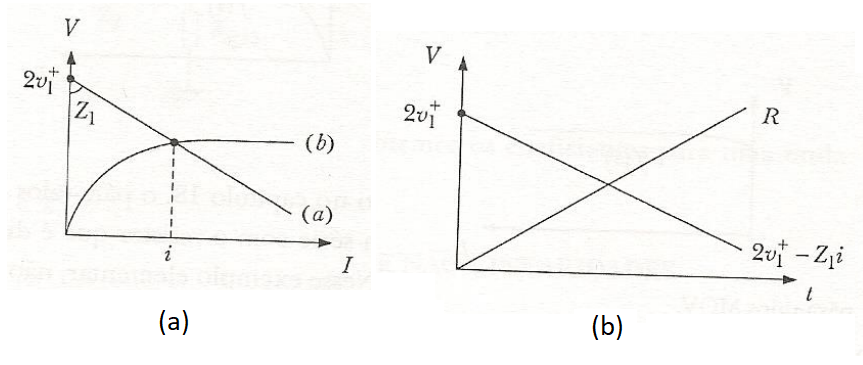
\includegraphics[width=8cm]{images/nlin2.png}
\caption{(a) solução gráfica e (b) terminação resistiva}
\label{slide7:nlin} 
\end{center}
\end{figure}

O método é comparado para o caso em que a casa é linear e $f(i) = Ri$.

A solução do problema não linear é abordado de várias formas, incluindo a linearização por partes da curva VxI do pára-raios. A escolha da quantidade de segmentos de reta pode variar de acordo com o esforço computacional desejado e o quão preciso será a resposta. Lembrando que quanto mais retas, mais precisa a solução, porém mais custosa.

Até agora a forma de onda da tensão incidente era considerada regular. Porém, as soluções traçadas anteriormente podem ser aplicadas para qualquer forma de onda.


